% -*- coding: UTF-8 -*-
% vim: autoindent expandtab tabstop=4 sw=4 sts=4 filetype=tex
% vim: spelllang=de spell
% chktex-file 27 - disable warning about missing include files

\subsection{Schatten}
\label{sec:rendering_implicit_surfaces_shadows}

Sofern im Text nicht anders vermerkt, basiert folgender Abschnitt
auf~\cite[S. 7]{reiner_smi_2011}.

Mittels Sphere Tracing können Schatten analog den vom Ray Tracing
bekannten Verfahren gewonnen werden. Dazu werden Schatten-Fühler oder
auch Schatten-Strahlen (``\textit{shadow rays}'') mit Sphere Tracing
abgetastet.  Man bildet also eine Folge von negativen Hüllkörpern
(``\textit{unbounding volumes}'') bzw. Kugeln (``\textit{unbounding
    spheres}'') pro Lichtquelle in Richtung dieser ausgehend von einem
Punkt einer Oberfläche. Die Folge wird so lange fortgesetzt, bis eine
Intersektion stattfindet oder bis eine definierte maximale Distanz
erreicht wurde.

Schatten-Fühler werden parametrisch als

\begin{gather}
    r_{s}(t) = \bm{x} + t \cdot r_{l}
\end{gather}

beschrieben. Wobei $r_{s}(t)$ der Ursprung des Schatten-Fühlers am Punkt $\bm{x}$
einer impliziten Oberfläche, $r_{l}$ die Richtung des Schatten-Fühlers
in Form eines Einheitsvektors und $t$ die zurückgelegte Distanz des
Strahles ist.

Der Algorithmus in~\autoref{alg:sphere_tracing_shadows} ist dem des
Sphere Tracings (siehe~\autoref{alg:sphere_tracing}) sehr ähnlich, der
Rückgabewert ist jedoch völlig verschieden. Der Algorithmus gibt den
Wert 1 zurück, wenn nach Erreichung der maximalen Distanz keine
Intersektion zwischen dem Schatten-Fühler und einer Oberfläche statt
fand.  Der Wert 0 wird zurückgegeben, wenn der Schatten-Fühler auf eine
Oberfläche getroffen ist und der Punkt $\bm{x}$ einer impliziten
Oberfläche sich daher im Schatten befindet.

\begin{lstlisting}[language=Python,caption={Algorithmus zur Berechnung
        von Schatten.},label={alg:sphere_tracing_shadows},captionpos=b,emph={calc_shadows}]
def calc_shadows():
    min_distance          = 0.01
    max_distance          = 9001
    shadow_ray_distance   = min_distance
    estimated_distance    = 0
    convergence_precision = 0.000001

    while shadow_ray_distance < max_distance:
        # sd_sphere is a signed distance function defining the implicit surface
        # cast_ray defines the ray equation given the current travelled /
        # marched distance of the ray
        estimated_distance = sd_sphere(cast_ray(shadow_ray_distance))

        if estimated_distance < convergence_precision:
            # the estimated distance is already smaller than the desired
            # precision of the convergence, so return zero (0) as we
            # have an intersection and therefore shadows
            return 0

        shadow_ray_distance = shadow_ray_distance + estimated_distance

    # When we reach this point, there was no intersection between the ray and a
    # implicit surface, so no shadows, so simply return 1
    return 1
\end{lstlisting}

Um zu verhindern, dass ein Punkt $\bm{x}$ einer impliziten Oberfläche
sich selbst verdeckt (sich also quasi selbst Schatten spendet), wird die
initial zurückgelegte Distanz (\textit{shadow\_ray\_distance}) auf einen
Minimalwert (\textit{min\_distance}) gesetzt. Dieser Wert sollte jedoch
wesentlich grösser als die gewünschte Präzision
(\textit{convergence\_precision}) sein, da ansonsten die Bedingung
(\textit{estimated\_distance < convergence\_precision}) ggf.\ initial
erfüllt und sich der Punkt $\bm{x}$ daher immer im Schatten befinden
würde.

\citeauthor{reiner_smi_2011} geben zudem an, wie weiche Schatten mittels
Sphere Tracing relativ einfach dargestellt werden können. Während der
Expansion anhand des Schatten-Fühlers wird die minimale, evaluierte
Distanz $d_{\text{min}}$ zu einem beliebigen Objekt gespeichert. Es wird
dabei angenommen, dass sich ein Punkt $\bm{x}$ einer impliziten
Oberfläche für schmale Distanzen $ 0 < d_{\text{min}} < d $ im Schatten
befindet. Somit ergibt schliesslich das Verhältnis der minimalen Distanz
zu der aktuellen Distanz einen Schatten- bzw.  Penumbra-Faktor:
$\text{shadow} = {d_{\text{min}} \over d}$, wobei $\text{shadow} \in (0,
1)$. Mit wachsender Distanz $d$ wächst auch die so genannte
Penumbra-Region.

Durch Speicherung der minimalen, evaluierten Distanz ist es möglich, die
Distanz des Schatten-Fühlers zu der ihn umgebenden Geometrie zu
untersuchen. Damit werden die Penumbra-Region sowie weiche Schatten
bestimmt. Befindet sich der Schatten-Fühler in der Nähe einer
Oberfläche ohne diese zu scheiden, ist die minimale Distanz
$d_{\text{min}}$ sehr gering. In diesem Fall, kann angenommen
werden, dass sich der Ursprungspunkt $\bm{x}$ in einer Penumbra-Region
befindet. Dies wiederum wirkt sich auf die Schattierung des Punktes aus: Je
knapper der Schatten-Fühler eine Oberfläche nicht geschnitten hat, desto
stärker wird der Punkt schattiert. Zusätzlich wird die Distanz des
Ursprungspunktes einbezogen. Je geringer diese ist, desto stärker wird
der Punkt schattiert.

Durch Hinzufügen eines Skalierungsfaktors kann ein Schattenwurf härter
oder weicher gezeichnet werden.

\begin{figure}[H]
    \centering
    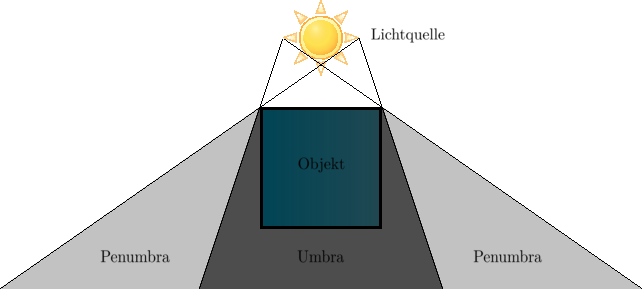
\includegraphics{img/shadowing.pdf}
    \caption{Illustration eines Schattenwurfes anhand einer Lichtquelle
        und einem Objekt. Im Bild sind die Umbra- und Penumbra-Regionen
        erkennbar.\protect\footnotemark}\label{fig:shadowing}
\end{figure}
\footnotetext{Eigene Darstellung mittels Inkscape, angelehnt
    an~\cite[S. 772]{glassner_introduction_1989}.}

\begin{lstlisting}[language=Python,caption={Algorithmus zur Berechnung
        von weichen Schatten.},label={alg:sphere_tracing_soft_shadows},captionpos=b,emph={calc_soft_shadows}]
def calc_soft_shadows():
    min_distance          = 0.01
    max_distance          = 9001
    shadow_ray_distance   = min_distance
    estimated_distance    = 0
    convergence_precision = 0.000001
    shadow                = 1.0
    scale                 = 32.0

    while shadow_ray_distance < max_distance:
        # sd_sphere is a signed distance function defining the implicit
        # surface, # cast_ray defines the ray equation given the current travelled /
        # marched distance of the ray
        estimated_distance = sd_sphere(cast_ray(shadow_ray_distance))

        if estimated_distance < convergence_precision:
            # the estimated distance is already smaller than the desired
            # precision of the convergence, so return zero (0) as we
            # have an intersection and therefore 'full' shadow
            return 0

        penumbra_factor = estimated_distance / shadow_ray_distance
        shadow = min(shadow, scale * penumbra_factor)
        shadow_ray_distance = shadow_ray_distance + estimated_distance

    # When we reach this point, there was no full intersection between
    # the ray and a implicit surface, so not entirely shadowed, so
    # return current shadow value
    return shadow
\end{lstlisting}
